%%%%%%%%%%%%%%%%%%%%%%%%%%%%%%%%%%%%%%%%%%%%%%%%%%%%%%%%%%%%%%%%%%%
%%%                                                             %%%
%%%      File: talk.tex                                         %%%
%%%    Author: Sabine Schulte im Walde                          %%%
%%%   Purpose: Research Seminar                                 %%%
%%%                                                             %%%
%%%%%%%%%%%%%%%%%%%%%%%%%%%%%%%%%%%%%%%%%%%%%%%%%%%%%%%%%%%%%%%%%%%


\documentclass[10pt]{beamer}


\usepackage{beamerthemesplit}
\usepackage[utf8]{inputenc}


\usetheme{Malmoe}
\usecolortheme{crane}
\useinnertheme{circles}

\title{Research Seminar}
\subtitle{An analysis of the NYC 311 Calls Dataset}

\author{Dhruv Mishra}
\institute{Master of Science \textit{Computational Linguistics}\\
  Institut für Maschinelle Sprachverarbeitung\\
  Universität Stuttgart}

\date{13/12/2018}


\begin{document}


\frame{\titlepage}


\begin{frame} \frametitle{Introduction}

  \begin{itemize}
    \item This report explores a small subset (about 250 MB+, as of 2015) of the database of complaints filed by residents of New York City since 2010 via 311 calls \cite{subset}.
    \item The full dataset is available at the NYC open data portal \cite{nycdatafull}.
\end{itemize}

\end{frame}

\begin{frame} \frametitle{Column Description}
The complete dataset has 41 columns but the subset considers only 6 of those columns, as described in \cite{nycdatafull}:

  \begin{itemize}
    \item Created Date: Date and Time when the complaint was created.
    \item Closed Date: Date and Time when the complaint was closed by responding agency.
    \item Agency: Acronym of responding City Government Agency.
    \item Complaint Type: This is the first level of a hierarchy identifying the topic of the incident or condition. Complaint Type may have a corresponding Descriptor or may stand alone.
    \item Descriptor: This is associated with the Complaint Type, and provides further detail on the incident or condition. Descriptor values are dependent on the Complaint Type and are not always required in a complaint.
    \item City: City of the incident location provided by geovalidation. These cities are actually the different neighbourhoods in NYC (for example Manhattan, Upper East Side, Brooklyn etc.) and should not be confused by the conventional definition of a city.
\end{itemize}

\end{frame}

\begin{frame} \frametitle{Preview of the data}
The top 5 rows of the database look like:

\begin{center}
 \begin{tabular}{||p{2.15cm} p{2.15cm} p{0.75cm} p{1.5cm} p{1.5cm} p{1cm}||}
 \hline
 Created Date & Closed Date & Agency & Complaint Type & Descriptor & City \\ [0.5ex]
 \hline\hline
 2015-09-15 02:14:04.000000 & None & NYPD & Illegal Parking & Blocked Hydrant & None \\
 \hline
 2015-09-15 02:12:49.000000 & None & NYPD & Noise - Street/Side walk & Loud Talking & NEW YORK \\
 \hline
 2015-09-15 02:11:19.000000 & None & NYPD & Noise - Street/Side walk & Loud Talking & NEW YORK \\
 \hline
 2015-09-15 02:09:46.000000 & None & NYPD & Noise - Commercial & Loud Talking & BRONX \\
 \hline
 2015-09-15 02:08:01.000000 & 2015-09-15 02:08:18.000000 & DHS & Homeless Person Assistance & Status Call  & NEW YORK \\ [1ex]
 \hline
\end{tabular}
\end{center}

\end{frame}

\begin{frame} \frametitle{Number of distinct values for each column}
The table below shows the number of distinct values present in each of the different columns.
\begin{center}
 \begin{tabular}{||c c||}
 \hline
 Column & Distinct Values \\ [0.5ex]
 \hline\hline
Agency    & 50 \\
Complaint Type    & 200 \\
Descriptor   & 1220 \\
City   & 547 \\ [1ex]
 \hline
\end{tabular}
\end{center}
\end{frame}

\begin{frame} \frametitle{What are the top 25 most common type of complaints?}
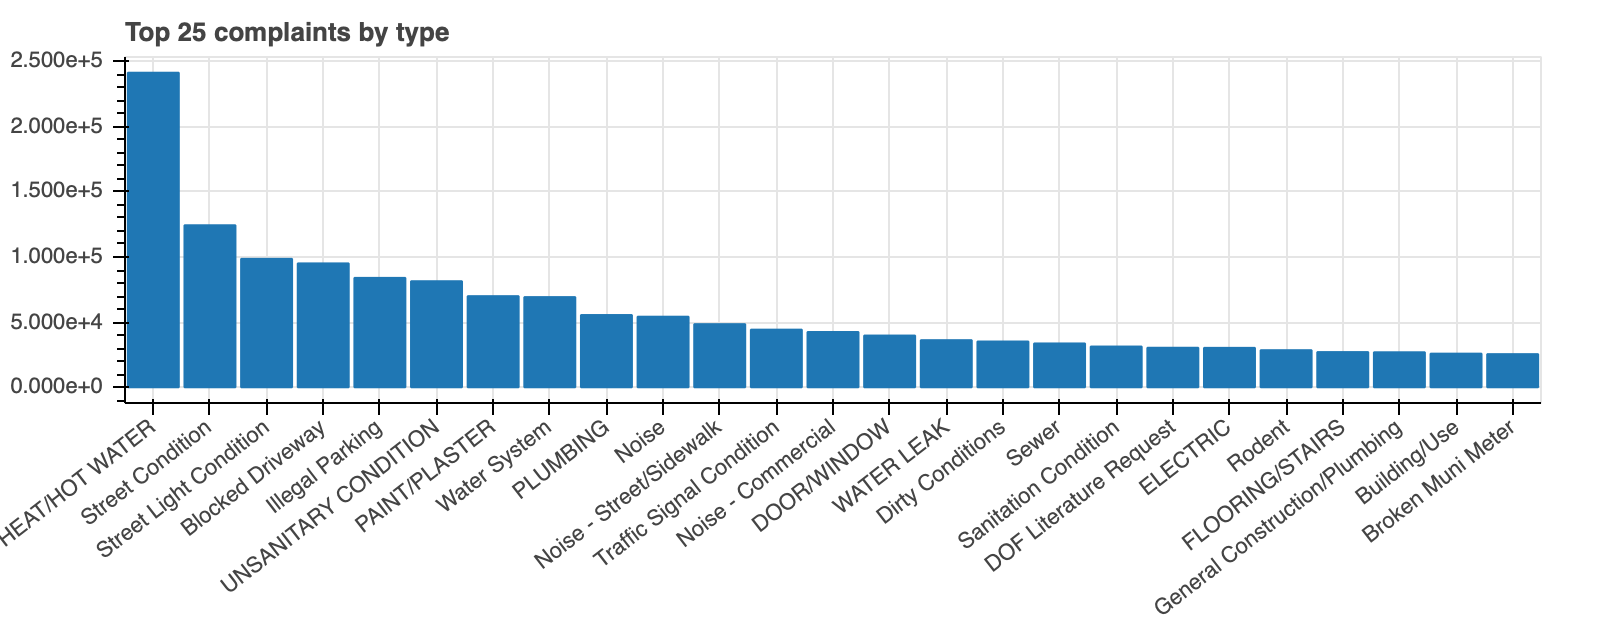
\includegraphics[scale=0.21]{top25complaints}
\end{frame}

\begin{frame} \frametitle{Top 10 cities with the largest number of complaints?}
\begin{center}
 \begin{tabular}{||c c||}
 \hline
 name & freq \\ [0.5ex]
 \hline\hline
BROOKLYN    & 579363 \\
NEW YORK    & 385655 \\
BRONX   & 342533 \\
STATEN ISLAND   & 92509 \\
Jamaica & 46683 \\
Flushing    & 35504 \\
ASTORIA & 31873 \\
Ridgewood   & 21618 \\
Woodside    & 15932 \\
Corona  & 15740 \\ [1ex]
 % 5 & 88 & 788 & 6344 \\ [1ex]
 \hline
\end{tabular}
\end{center}
\end{frame}


\begin{frame} \frametitle{What is the number of complaints by type and by city for the top 7 cities?}
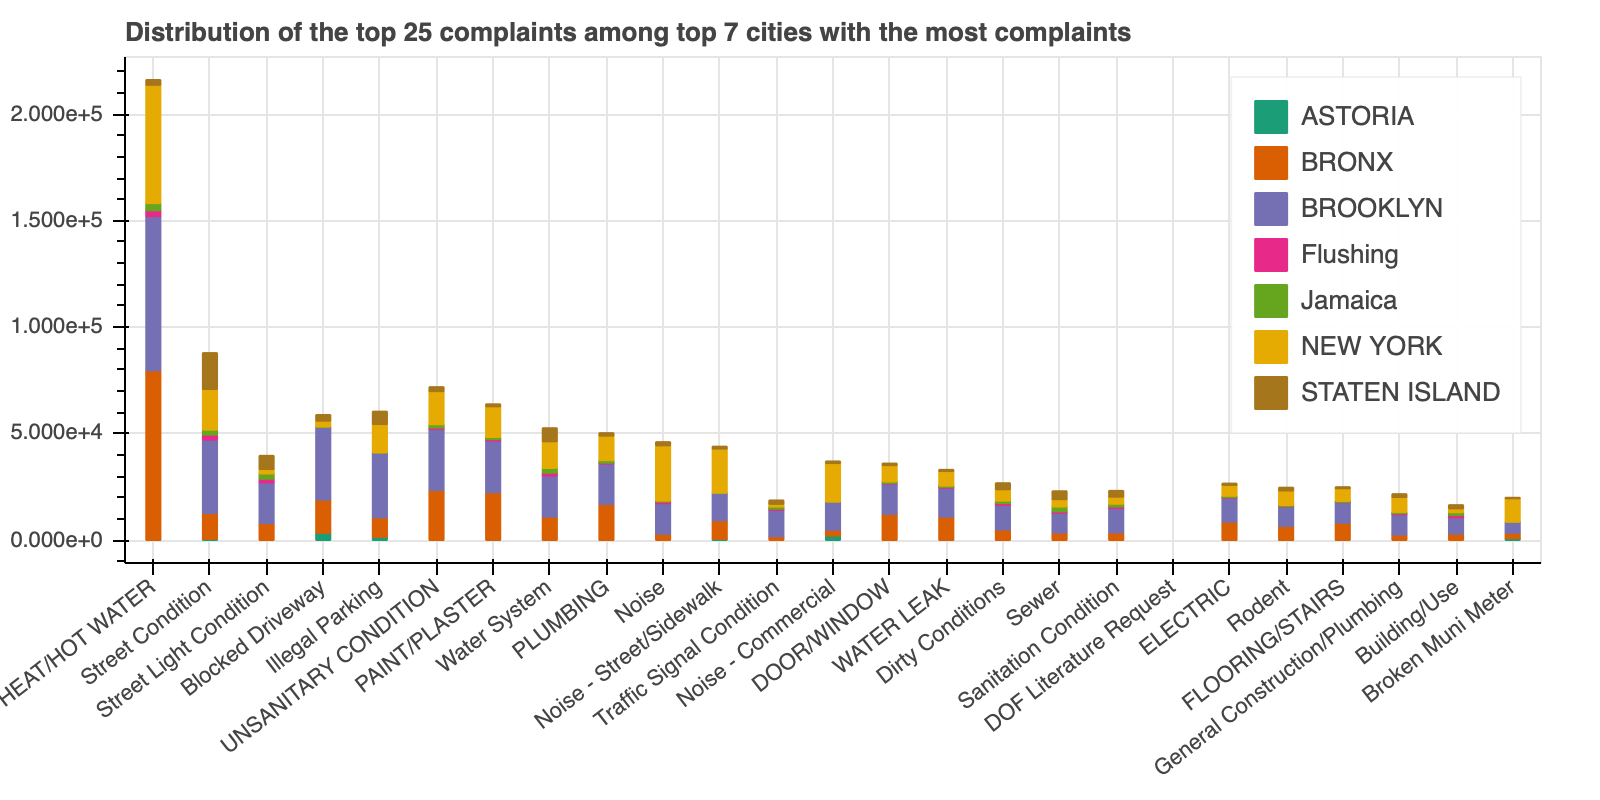
\includegraphics[scale=0.21]{topcomplaintsfortop7cities}
\end{frame}

\begin{frame} \frametitle{What is the most common hour for noise complaints?}
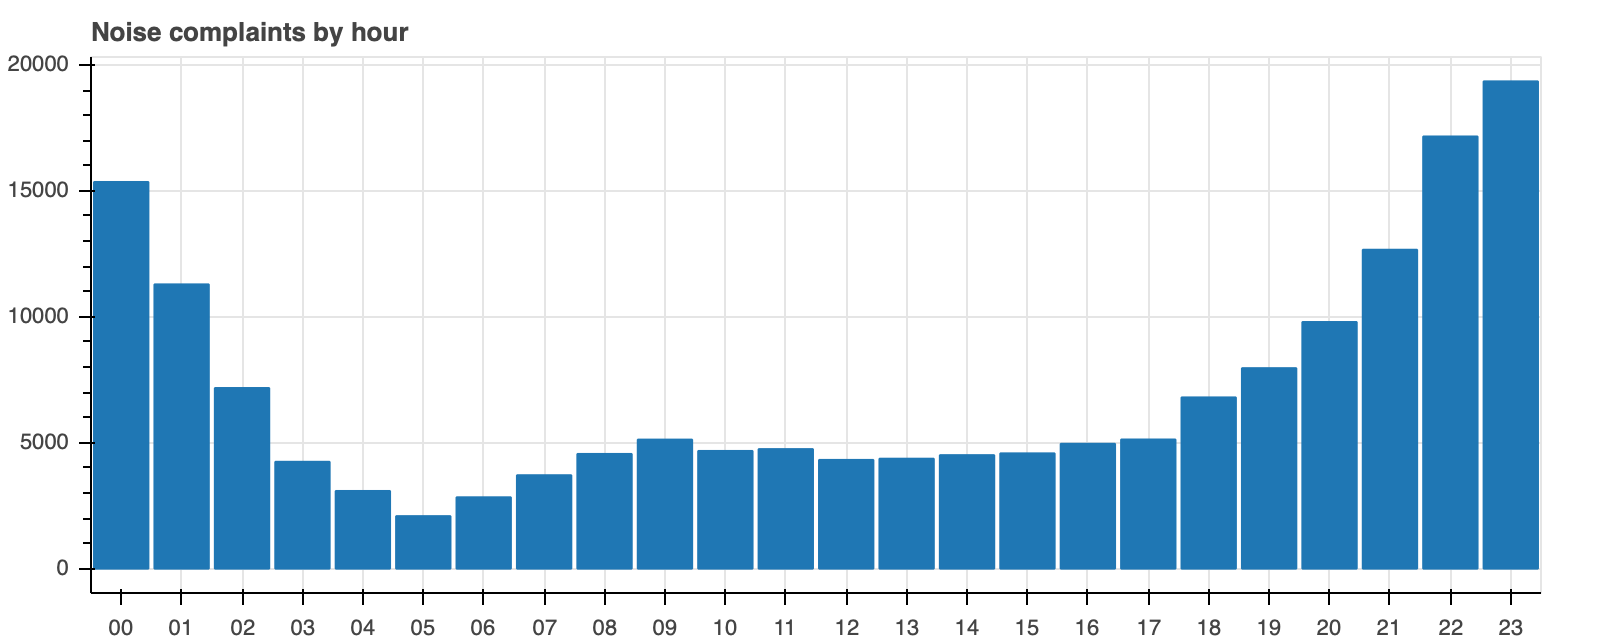
\includegraphics[scale=0.21]{noisecomplaintsbyhour}
\end{frame}



\begin{frame} \frametitle{Timeseries for top 5 complaints}
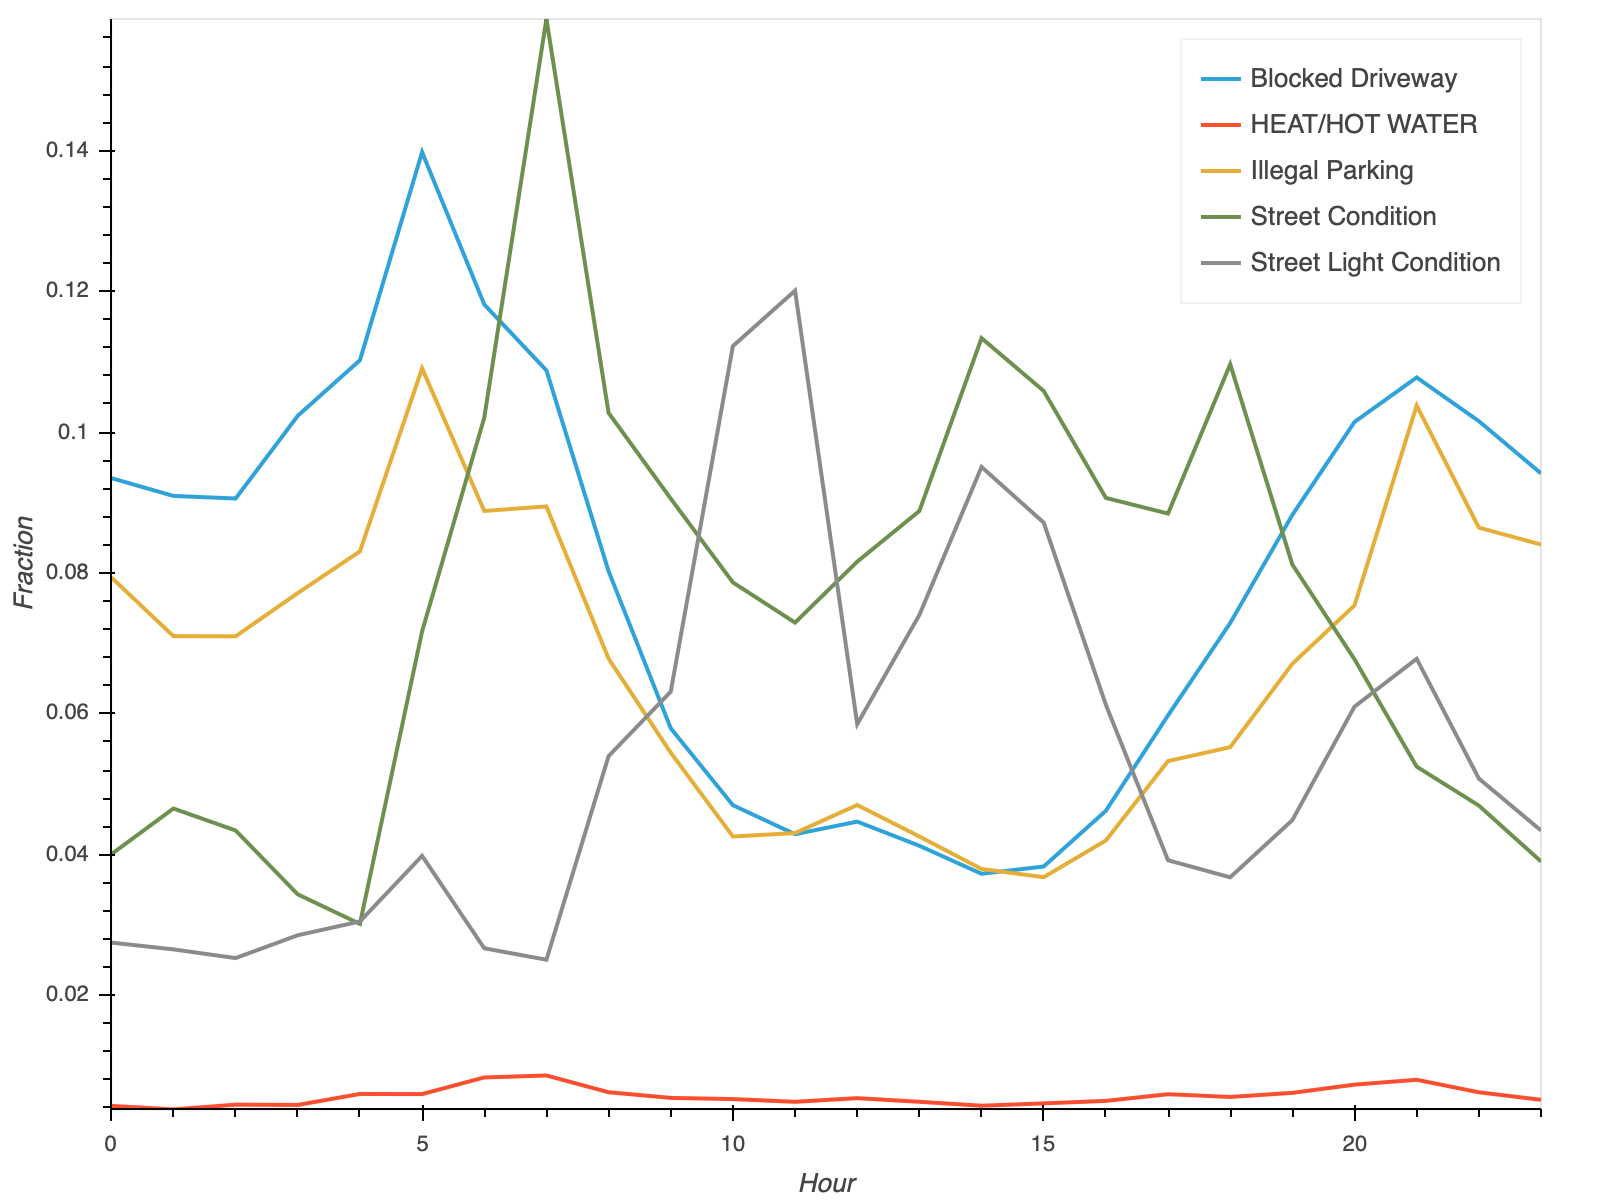
\includegraphics[scale=0.17]{timeseries}

A line chart for showing the fraction of complaints (y-axis) associated with each hour of the day (x-axis)
\end{frame}

\begin{frame} \frametitle{References}
% Bibliography:
\begin{thebibliography}{9}
\bibitem{nycdatafull}
NYC Open Data
\\\texttt{https://nycopendata.socrata.com/Social-Services/311-Service\\-Requests-from-2010-to-Present/erm2-nwe9}

\bibitem{subset}
NYC Open Data Subset used in this report
\\\texttt{https://onedrive.live.com/download?cid=FD520DDC6BE92730\&\\resid=FD520DDC6BE92730\%21616\&authkey=AEeP\_4E1uh-vyDE}

\bibitem{plotly}
Big data analytics using python and sqlite on NYC's 311 complaints since 2003.
\\\texttt{https://plot.ly/ipython-notebooks/big-data-\\analytics-with-pandas-and-sqlite/}


\bibitem{online}
Open online course in python
\\\texttt{https://www.edx.org/course/introduction-to-computing\\-for-data-analysis-2}

\end{thebibliography}

\end{frame}

\end{document}


%% --- END OF FILE
